\documentclass{../../ktane-mod}
\RequirePackage{multicol}


\begin{document}

\begin{module}{
  moduleName=Morse Code,
  indexString=Morse Code,
  imageResource=morse_code_img.pdf,
  interactions=\keysymbol
}{
  An antiquated form of naval communication?
  What next?
  At least it's genuine Morse Code, so pay attention and you might just learn something.
}
  \begin{bulletlist}
    \bulletitem{Interpret the signal from the flashing light using the Morse Code chart on the next page.}
    \bulletitem{The signal will loop, with a long gap between repetitions.}
    \bulletitem{Identify the word that is being signaled.}
    \bulletitem{Once the word is identified, adjust the response frequency of the module as indicated in the table on the last page and press the transmit (TX) button.}
    \bulletitem{Refer to the next double-page for defusing the module.}
  \end{bulletlist}

  \textheading{Morse Code Mnemonic}

  \YELLOW[Ignore this if you aren't here to learn Morse Code.]

  The words below show each Morse Code letter in a graphic form.
  Letters deviating from the base line signify a \LIGHTBLUE[dash], others a \LIGHTRED[dot].
  \begin{multicols}{3}
    A --- \LIGHTRED[a]\LIGHTBLUE[t]

    B --- \LIGHTBLUE[b]\LIGHTRED[e]\LIGHTRED[a]\LIGHTRED[n]

    C --- \LIGHTBLUE[C]\LIGHTRED[a]\LIGHTBLUE[t]\LIGHTRED[e]

    D --- \LIGHTBLUE[d]\LIGHTRED[a]\LIGHTRED[m]

    E --- \LIGHTRED[e]

    F --- \LIGHTRED[c]\LIGHTRED[a]\LIGHTBLUE[f]\LIGHTRED[e]

    G --- \LIGHTBLUE[g]\LIGHTBLUE[y]\LIGHTRED[m]

    H --- \LIGHTRED[e]\LIGHTRED[a]\LIGHTRED[r]\LIGHTRED[s] (hear)

    I --- \LIGHTRED[i]\LIGHTRED[n]

    J --- \LIGHTRED[e]\LIGHTBLUE[d]\LIGHTBLUE[g]\LIGHTBLUE[y] (\textbackslash\ 'e-j\=e \textbackslash)

    K --- \LIGHTBLUE[K]\LIGHTRED[i]\LIGHTBLUE[t](-Kat)

    L --- \LIGHTRED[e]\LIGHTBLUE[l]\LIGHTRED[s]\LIGHTRED[e]

    M --- \LIGHTBLUE[M]\LIGHTBLUE[M] \,(Millenia)

    N --- \LIGHTBLUE[N]\LIGHTRED[o]

    O --- \LIGHTBLUE[O]\LIGHTBLUE[O]\LIGHTBLUE[P] (Object Oriented Programming)

    P --- \LIGHTRED[a]\LIGHTBLUE[p]\LIGHTBLUE[p]\LIGHTRED[s]

    Q --- \LIGHTBLUE[p]\LIGHTBLUE[l]\LIGHTRED[a]\LIGHTBLUE[q](ue)

    R --- \LIGHTRED[r]\LIGHTBLUE[y]\LIGHTRED[e]

    S --- \LIGHTRED[s]\LIGHTRED[a]\LIGHTRED[x]

    T --- (Mr) \LIGHTBLUE[T]

    U --- \LIGHTRED[u]\LIGHTRED[m]\LIGHTBLUE[p](ire)

    V --- \LIGHTRED[v]\LIGHTRED[e]\LIGHTRED[a]\LIGHTBLUE[l]

    W --- \LIGHTRED[w]\LIGHTBLUE[h]\LIGHTBLUE[y]

    X --- \LIGHTBLUE[f]\LIGHTRED[o]\LIGHTRED[x]\LIGHTBLUE[y]

    Y --- \LIGHTBLUE[y]\LIGHTRED[e]\LIGHTBLUE[l]\LIGHTBLUE[l]

    Z --- \LIGHTBLUE[Z]\LIGHTBLUE[h]\LIGHTRED[o]\LIGHTRED[u] (Province in China)
  \end{multicols}

  \clearpage

\textheading{Morse Code Alphabet Tree}

  \newcommand{\mdot}{{\Large •}}
  \newcommand{\mdash}{{\Large -}}

  This tree shows the complete morse alphabet.
  Navigate it as the defuser tells you individual Morse symbols.
  Letters marked in \RED[red] do not appear in any of the solution words.
  Letters marked in \LIGHTGREEN[green] are unique to a single solution word.

  \begin{bulletlist}
    \bulletitem{If the defuser sees a short flash (dot / •), move up and to the right.}
    \bulletitem{If the defuser sees a long flash (dash / -), move down and to the right.}
    \bulletitem{If the defuser sees a gap, read the letter at the current position.}
  \end{bulletlist}

\begin{center}
\begin{tikzpicture}[grow=right, level distance=40mm,
level 1/.style={sibling distance=112mm},
level 2/.style={sibling distance=56mm},
level 3/.style={sibling distance=28mm},
level 4/.style={sibling distance=14mm},
scale=1]
\node {\Large}
    child { node {\Large T}
        child { node {\Large\LIGHTGREEN[M]}
            child { node {\Large O}
                edge from parent node[below=1mm] {\mdash}
            }
            child { node {\Large\LIGHTGREEN[G]}
                child { node {\Large\RED[Q]}
                    edge from parent node[below=1mm] {\mdash}
                }
                child { node {\Large\RED[Z]}
                    edge from parent node[above] {\mdot}
                }
                edge from parent node[above] {\mdot}
            }
            edge from parent node[below=1mm] {\mdash}
        }
        child { node {\Large\LIGHTGREEN[N]}
            child { node {\Large K}
                child { node {\Large\RED[Y]}
                    edge from parent node[below=1mm] {\mdash}
                }
                child { node {\Large C}
                    edge from parent node[above] {\mdot}
                }
                edge from parent node[below=1mm] {\mdash}
            }
            child { node {\Large\RED[D]}
                child { node {\Large\LIGHTGREEN[X]}
                    edge from parent node[below=1mm] {\mdash}
                }
                child { node {\Large B}
                    edge from parent node[above] {\mdot}
                }
                edge from parent node[above] {\mdot}
            }
            edge from parent node[above] {\mdot}
        }
        edge from parent node[below=2mm] {\mdash}
    }
    child { node {\Large E}
        child { node {\Large A}
            child { node {\Large\RED[W]}
                child { node {\Large\RED[J]}
                    edge from parent node[below=1mm] {\mdash}
                }
                child { node {\Large\RED[P]}
                    edge from parent node[above] {\mdot}
                }
                edge from parent node[below=1mm] {\mdash}
            }
            child { node {\Large R}
                child { node {\Large L}
                    edge from parent node[above] {\mdot}
                }
                edge from parent node[above] {\mdot}
            }
            edge from parent node[below=1mm] {\mdash}
        }
        child { node {\Large I}
            child { node {\Large\RED[U]}
                child { node {\Large\LIGHTGREEN[F]}
                    edge from parent node[above] {\mdot}
                }
                edge from parent node[below=1mm] {\mdash}
            }
            child { node {\Large S}
                child { node {\Large\LIGHTGREEN[V]}
                    edge from parent node[below=1mm] {\mdash}
                }
                child { node {\Large H}
                    edge from parent node[above] {\mdot}
                }
                edge from parent node[above] {\mdot}
            }
            edge from parent node[above] {\mdot}
        }
        edge from parent node[above=1mm] {\mdot}
    };
\end{tikzpicture}
\end{center}

\newpage

\textheading{Word Recognition Trees}

If you identify any letter in the signal, start at the corresponding tree below.
It shows the possible continuations after the identified letter, thereby allowing to identify the target word as quickly as possible.
The trees are built such that the long gap between signal repetitions can be ignored.

\begin{multicols}{3}
\raggedright

% Tree for 'a'
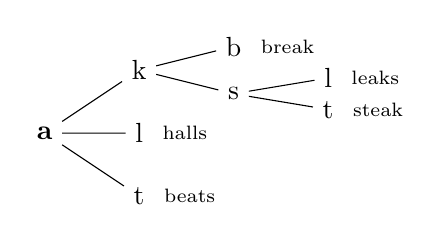
\begin{tikzpicture}[grow=right, level distance=12mm, sibling distance=8mm,
  level 1/.style={sibling distance=8mm},
  level 2/.style={sibling distance=6mm},
  level 3/.style={sibling distance=4mm},
  scale=1.0]
\node {\textbf{a}}
    child { node[label=right:\scriptsize beats] {t} }
    child { node[label=right:\scriptsize halls] {l} }
    child { node {k}
        child { node {s}
            child { node[label=right:\scriptsize steak] {t} }
            child { node[label=right:\scriptsize leaks] {l} }
        }
        child { node[label=right:\scriptsize break] {b} }
    };
\end{tikzpicture}

\vspace{5mm}

% Tree for 'b'
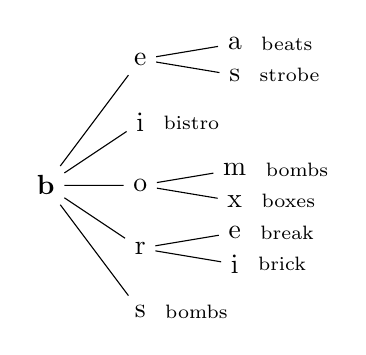
\begin{tikzpicture}[grow=right, level distance=12mm, sibling distance=4mm,
level 1/.style={sibling distance=8mm},
level 2/.style={sibling distance=4mm},
scale=1.0]
\node {\textbf{b}}
    child { node[label=right:\scriptsize bombs] {s} }
    child { node {r}
        child { node[label=right:\scriptsize brick] {i} }
        child { node[label=right:\scriptsize break] {e} }
    }
    child { node {o}
        child { node[label=right:\scriptsize boxes] {x} }
        child { node[label=right:\scriptsize bombs] {m} }
    }
    child { node[label=right:\scriptsize bistro] {i} }
    child { node {e}
        child { node[label=right:\scriptsize strobe] {s} }
        child { node[label=right:\scriptsize beats] {a} }
    };
\end{tikzpicture}

\vspace{5mm}

% Tree for 'c'
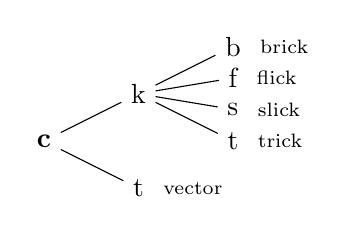
\begin{tikzpicture}[grow=right, level distance=12mm, sibling distance=4mm,
level 1/.style={sibling distance=12mm},
level 2/.style={sibling distance=4mm},
scale=1.0]
\node {\textbf{c}}
    child { node[label=right:\scriptsize vector] {t} }
    child { node {k}
        child { node[label=right:\scriptsize trick] {t} }
        child { node[label=right:\scriptsize slick] {s} }
        child { node[label=right:\scriptsize flick] {f} }
        child { node[label=right:\scriptsize brick] {b} }
    };
\end{tikzpicture}

\vspace{5mm}

% Tree for 'e'
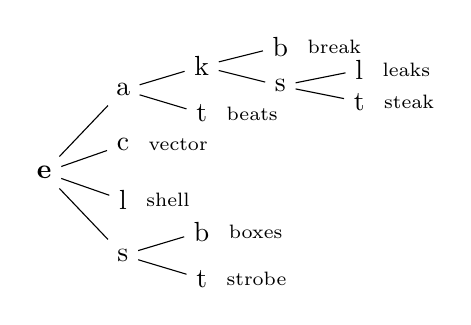
\begin{tikzpicture}[grow=right, level distance=10mm, sibling distance=4mm,
level 1/.style={sibling distance=7mm},
level 2/.style={sibling distance=6mm},
level 3/.style={sibling distance=5mm},
level 4/.style={sibling distance=4mm},
scale=1.0]
\node {\textbf{e}}
    child { node {s}
        child { node[label=right:\scriptsize strobe] {t} }
        child { node[label=right:\scriptsize boxes] {b} }
    }
    child { node[label=right:\scriptsize shell] {l} }
    child { node[label=right:\scriptsize vector] {c} }
    child { node {a}
        child { node[label=right:\scriptsize beats] {t} }
        child { node {k}
            child { node {s}
                child { node[label=right:\scriptsize steak] {t} }
                child { node[label=right:\scriptsize leaks] {l} }
            }
            child { node[label=right:\scriptsize break] {b} }
        }
    };
\end{tikzpicture}

\vspace{5mm}

% Tree for 'f'
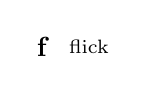
\begin{tikzpicture}[grow=right, level distance=12mm, sibling distance=8mm, scale=1.0]
\node[label=right:\scriptsize flick] {\textbf{f}};
\end{tikzpicture}

\vspace{5mm}

% Tree for 'g'
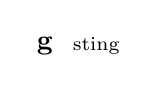
\begin{tikzpicture}[grow=right, level distance=12mm, sibling distance=8mm, scale=1.0]
\node[label=right:\scriptsize sting] {\textbf{g}};
\end{tikzpicture}

\vspace{5mm}

% Tree for 'h'
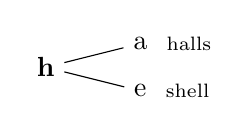
\begin{tikzpicture}[grow=right, level distance=12mm, sibling distance=6mm, scale=1.0]
\node {\textbf{h}}
    child { node[label=right:\scriptsize shell] {e} }
    child { node[label=right:\scriptsize halls] {a} };
\end{tikzpicture}

\vspace{5mm}

% Tree for 'i'
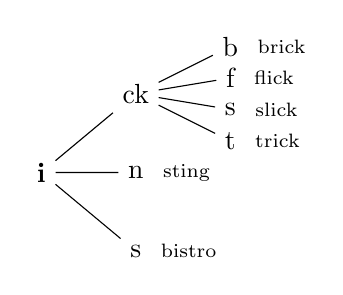
\begin{tikzpicture}[grow=right, level distance=12mm, sibling distance=4mm,
level 1/.style={sibling distance=10mm},
level 2/.style={sibling distance=4mm},
scale=1.0]
\node {\textbf{i}}
    child { node[label=right:\scriptsize bistro] {s} }
    child { node[label=right:\scriptsize sting] {n} }
    child { node {ck}
        child { node[label=right:\scriptsize trick] {t} }
        child { node[label=right:\scriptsize slick] {s} }
        child { node[label=right:\scriptsize flick] {f} }
        child { node[label=right:\scriptsize brick] {b} }
    };
\end{tikzpicture}

\vspace{5mm}

\columnbreak

% Tree for 'k'
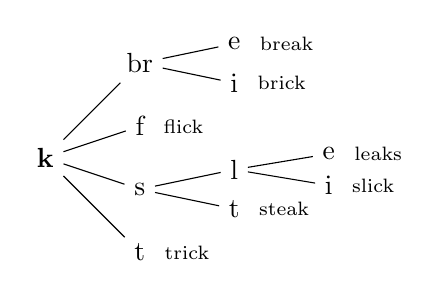
\begin{tikzpicture}[grow=right, level distance=12mm, sibling distance=4mm,
level 1/.style={sibling distance=8mm},
level 2/.style={sibling distance=5mm},
level 3/.style={sibling distance=4mm},
scale=1.0]
\node {\textbf{k}}
    child { node[label=right:\scriptsize trick] {t} }
    child { node {s}
        child { node[label=right:\scriptsize steak] {t} }
        child { node {l}
            child { node[label=right:\scriptsize slick] {i} }
            child { node[label=right:\scriptsize leaks] {e} }
        }
    }
    child { node[label=right:\scriptsize flick] {f} }
    child { node {br}
        child { node[label=right:\scriptsize brick] {i} }
        child { node[label=right:\scriptsize break] {e} }
    };
\end{tikzpicture}

\vspace{5mm}

% Tree for 'l'
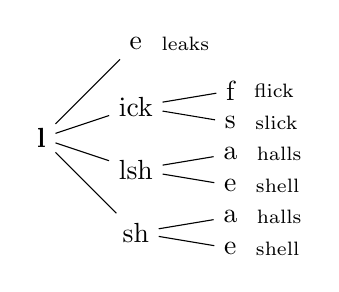
\begin{tikzpicture}[grow=right, level distance=12mm, sibling distance=4mm,
level 1/.style={sibling distance=8mm},
level 2/.style={sibling distance=4mm},
scale=1.0]
\node {\textbf{l}}
    child { node {sh}
        child { node[label=right:\scriptsize shell] {e} }
        child { node[label=right:\scriptsize halls] {a} }
    }
    child { node {lsh}
        child { node[label=right:\scriptsize shell] {e} }
        child { node[label=right:\scriptsize halls] {a} }
    }
    child { node {ick}
        child { node[label=right:\scriptsize slick] {s} }
        child { node[label=right:\scriptsize flick] {f} }
    }
    child { node[label=right:\scriptsize leaks] {e} };
\end{tikzpicture}

\vspace{5mm}

% Tree for 'm'
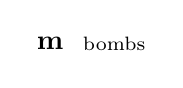
\begin{tikzpicture}[grow=right, level distance=12mm, sibling distance=8mm, scale=1.0]
\node[label=right:\scriptsize bombs] {\textbf{m}};
\end{tikzpicture}

\vspace{5mm}

% Tree for 'n'
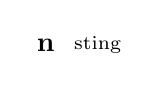
\begin{tikzpicture}[grow=right, level distance=12mm, sibling distance=8mm, scale=1.0]
\node[label=right:\scriptsize sting] {\textbf{n}};
\end{tikzpicture}

\vspace{5mm}

% Tree for 'o'
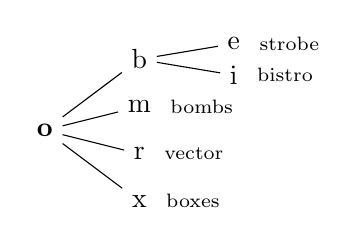
\begin{tikzpicture}[grow=right, level distance=12mm, sibling distance=4mm,
level 1/.style={sibling distance=6mm},
level 2/.style={sibling distance=4mm},
scale=1.0]
\node {\textbf{o}}
    child { node[label=right:\scriptsize boxes] {x} }
    child { node[label=right:\scriptsize vector] {r} }
    child { node[label=right:\scriptsize bombs] {m} }
    child { node {b}
        child { node[label=right:\scriptsize bistro] {i} }
        child { node[label=right:\scriptsize strobe] {e} }
    };
\end{tikzpicture}

\vspace{5mm}

% Tree for 'r'
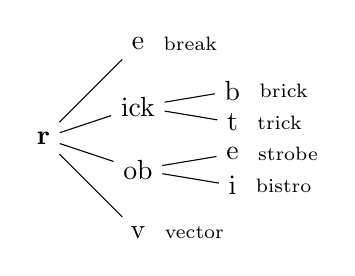
\begin{tikzpicture}[grow=right, level distance=12mm, sibling distance=4mm,
level 1/.style={sibling distance=8mm},
level 2/.style={sibling distance=4mm},
scale=1.0]
\node {\textbf{r}}
    child { node[label=right:\scriptsize vector] {v} }
    child { node {ob}
        child { node[label=right:\scriptsize bistro] {i} }
        child { node[label=right:\scriptsize strobe] {e} }
    }
    child { node {ick}
        child { node[label=right:\scriptsize trick] {t} }
        child { node[label=right:\scriptsize brick] {b} }
    }
    child { node[label=right:\scriptsize break] {e} };
\end{tikzpicture}

\vspace{5mm}

% Tree for 's'
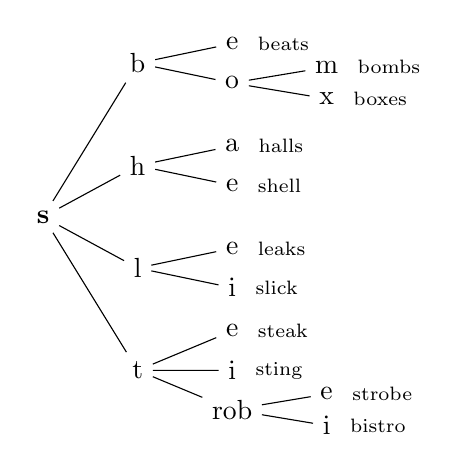
\begin{tikzpicture}[grow=right, level distance=12mm, sibling distance=4mm,
level 1/.style={sibling distance=13mm},
level 2/.style={sibling distance=5mm},
level 3/.style={sibling distance=4mm},
scale=1.0]
\node {\textbf{s}}
    child { node {t}
        child { node {rob}
            child { node[label=right:\scriptsize bistro] {i} }
            child { node[label=right:\scriptsize strobe] {e} }
        }
        child { node[label=right:\scriptsize sting] {i} }
        child { node[label=right:\scriptsize steak] {e} }
    }
    child { node {l}
        child { node[label=right:\scriptsize slick] {i} }
        child { node[label=right:\scriptsize leaks] {e} }
    }
    child { node {h}
        child { node[label=right:\scriptsize shell] {e} }
        child { node[label=right:\scriptsize halls] {a} }
    }
    child { node {b}
        child { node {o}
            child { node[label=right:\scriptsize boxes] {x} }
            child { node[label=right:\scriptsize bombs] {m} }
        }
        child { node[label=right:\scriptsize beats] {e} }
    };
\end{tikzpicture}

\vspace{5mm}

\columnbreak

% Tree for 't'
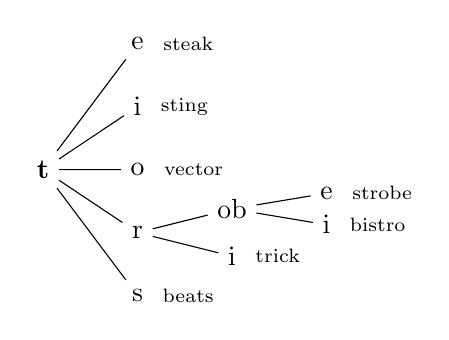
\begin{tikzpicture}[grow=right, level distance=12mm, sibling distance=4mm,
level 1/.style={sibling distance=8mm},
level 2/.style={sibling distance=6mm},
level 3/.style={sibling distance=4mm},
scale=1.0]
\node {\textbf{t}}
    child { node[label=right:\scriptsize beats] {s} }
    child { node {r}
        child { node[label=right:\scriptsize trick] {i} }
        child { node {ob}
            child { node[label=right:\scriptsize bistro] {i} }
            child { node[label=right:\scriptsize strobe] {e} }
        }
    }
    child { node[label=right:\scriptsize vector] {o} }
    child { node[label=right:\scriptsize sting] {i} }
    child { node[label=right:\scriptsize steak] {e} };
\end{tikzpicture}

\vspace{5mm}

% Tree for 'v'

\begin{tikzpicture}[grow=right, level distance=12mm, sibling distance=8mm, scale=1.0]
\node[label=right:\scriptsize vector] {\textbf{v}};
\end{tikzpicture}

\vspace{5mm}

% Tree for 'x'
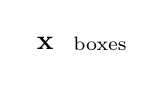
\begin{tikzpicture}[grow=right, level distance=12mm, sibling distance=8mm, scale=1.0]
\node[label=right:\scriptsize boxes] {\textbf{x}};
\end{tikzpicture}

\vspace{12mm}

\textheading{Response Frequencies}

Each word corresponds to a specific response frequency:

\renewcommand{\arraystretch}{1.5}
\begin{center}
\begin{NiceTabular}{
 >{\centering\arraybackslash}m{2cm}
 >{\centering\arraybackslash}m{2cm}
}[hvlines]
\textbf{If the word is:} & \textbf{Respond at frequency:} \\
beats  & 3.600 MHz\\
bistro & 3.552 MHz\\
bombs  & 3.565 MHz\\
boxes  & 3.535 MHz\\
break  & 3.572 MHz\\
brick  & 3.575 MHz\\
flick  & 3.555 MHz\\
halls  & 3.515 MHz\\
leaks  & 3.542 MHz\\
shell  & 3.505 MHz\\
slick  & 3.522 MHz\\
steak  & 3.582 MHz\\
sting  & 3.592 MHz\\
strobe & 3.545 MHz\\
trick  & 3.532 MHz\\
vector & 3.595 MHz\\
\end{NiceTabular}
\end{center}

\end{multicols}

\end{module}

\end{document}
